\documentclass{article}

\usepackage[utf8]{inputenc}
\usepackage[russian]{babel}
\usepackage{graphicx}
\graphicspath{{results/}}
\DeclareGraphicsExtensions{.pdf,.png,.jpg}
\usepackage[unicode, pdftex]{hyperref}
\usepackage{csvsimple}
\usepackage[stable]{footmisc}
\usepackage{subfigure}
\usepackage{indentfirst}


\begin{document}

\begin{titlepage}
  \centerline {Санкт-Петербургский политехнический университет}
  \centerline { им. Петра Великого}
  \centerline { }
  \centerline {Институт прикладной математики и механики} 
  \centerline {Кафедра "Прикладная математика"}
  \vfill
  \centerline{\textbf{Отчёт}}
  \centerline{\textbf{по лабораторной работе №5}}
  \centerline{\textbf{по дисциплине}}
  \centerline{\textbf{"Математическая статистика"}}
  \vfill
  \hfill
  \begin{minipage}{0.45\textwidth}
  Выполнил студент:\\
  Дроздова Дарья Александровна\\
  группа: 3630102/80401 \\
  \\
  Проверил:\\
  к.ф.-м.н., доцент \\
  Баженов Александр Николаевич
  \end{minipage}
  \vfill
  \centerline {Санкт-Петербург}   
  \centerline {2021 г.}  
\end{titlepage}

\newpage
\setcounter{page}{2}
\tableofcontents

\newpage
\listoffigures

\newpage
\listoftables

\newpage
\section{Постановка задачи}

Сгенерировать двумерные выборки для нормального распределения мощности 20, 60 и 100 элементов. Коэффициент корреляции $\rho$ взять равным 0, 0.5, 0.9.

Сгенерировать выборки 1000 раз и вычислить следующие средние значение, среднее значение квадрата и дисперсия для следующих параметров:
\begin{itemize}
	\item Коэффициент корреляции Пирсона
	\item Коэффициент корреляции Спирмена
	\item Квадратного коэффициента корреляции
\end{itemize}

Аналогичные вычисления сделать для смеси нормальных распределений:
\begin{equation}
f(x,y) = 0.9 N(x,y,0,0,1,1,0.9) + 0.1 N(x,y,0,0,10,10,-0.9)
\label{eq:1}
\end{equation}

Для нормального распределения построить сгенерированные точки на плоскости и построить эллипс равновероятности.

\newpage
\section{Теория}

\subsection{Двумерное нормальное распределение}

Двумерная случайная величина $(X,Y)$ называется распределенной нормально, если ее плотность вероятности определена формулой \\


$
N(x,y,\overline{x}, \overline{y}, \sigma_x, \sigma_y, \rho) = \frac{1}{2\pi\sigma_x\sigma_y\sqrt{1-\rho^2}} \times $
\begin{equation}
\times \exp \left\{ -\frac{1}{2(1-\rho^2)} \left[ \frac{(x-\overline{x})^2}{\sigma_x^2} - 2\rho\frac{(x-\overline{x})(y-\overline{y})}{\sigma_x\sigma_y} + \frac{(y-\overline{y})^2}{\sigma_2^2} \right] \right\}
\label{eq:2}
\end{equation}
где $X,Y$ - нормально распределенные случайные величины с математическим ожиданием $\overline{x}, \overline{y}$ и средними квадратичными отклонениями $\sigma_x, \sigma_y$ соответственно, $\rho$ - коэффициент корреляции.

\subsection{Корреляционный момент и коэффициент корреляции}

Корреляционный момент (ковариация) двух случайных величин $X, Y$ определяется по следующей формуле
$$
K = cov(X,Y) = M[(X - \overline{x})(Y - \overline{y})]
$$ 
т. е. данная величина определяется как математическое ожидание произведения отклонений случайных величин от их математических ожиданий.

Коэффициент корреляции $\rho$ определяется по следующей формуле
$$
\rho = \frac{K}{\sigma_x\sigma_y}
$$
 
Коэффициент корреляции - это нормированная числовая характеристика, которая является мерой близости зависимости между случайными величинами к линейной.

\subsection{Выборочные коэффициенты корреляции}

\subsubsection{Выборочный коэффициент корреляции Пирсона}

Естественной оценкой для $\rho$ служит его статистический аналог в виде выборочного коэффициента корреляции, предложенный К. Пирсоном
\begin{equation}
r = \frac{\sum (x_i - \overline{x})(y_i - \overline{y})}{\sqrt{\sum (x_i - \overline{x})^2 \sum(y_i - \overline{y})^2}} = \frac{K}{s_X s_Y}
\label{eq:3}
\end{equation}
где $K$ - выборочная ковариация, $s_X^2, s_Y^2$ - выборочная дисперсия случайных величин $X$ и $Y$ соответственно.

\subsubsection{Выборочный квадратный коэффициент корреляции}

Выборочный квадратный коэффициент корреляции определяется по следующей формуле 
\begin{equation}
r_Q = \frac{n_1 + n_3 - n_2 - n_4}{n}
\label{eq:4}
\end{equation}
где $n_1, n_2, n_3, n_4$ - количество точек с координатами $(x_i, y_i)$, попавшим соответственно в I, II, III и IV квадранты декартовой системы с осями $x' = x - \mathrm{med}\;x, y' = y - \mathrm{med}\;y$ и с центом в точке с координатами $(\mathrm{med}\;x, \mathrm{med}\;y)$
\begin{figure}[h]
\center{\includegraphics[scale=0.5]{axes}}
\end{figure}

\subsubsection{Выборочный коэффициент ранговой корреляции Спирмена}

Выриационный ряд  - последовательность значений выборки $X = (x_1,...,x_n)$б расположенных в порядке неубывания
$$
x^{(1)} \le x^{(2)} \le ... \le x^{(n)}
$$
Рангом $r_i$ наблюдения $x_i$ называется его порядковый номер  в вариационном ряду
$$
x^{(r_i)} = x_i
$$

Выборочный коэффициент ранговой корреляции Спирмена определяется по формуле 
\begin{equation}
r = \frac{\sum (u_i - \overline{u})(v_i - \overline{v})}{\sqrt{\sum (u_i - \overline{u})^2 \sum(v_i - \overline{v})^2}}
\label{eq:5}
\end{equation}
где $\overline{u} = \overline{v} = \frac{n + 1}{2}$ - среднее значение рангов, $u$ - ранги, соответствующие значениям переменной $X$, $v$ - ранги, соответствующие значениям переменной $Y$.


\subsection{Эллипс рассеивания}

Рассмотрим поверхность распределения (\ref{eq:2}). Она имеет вид холма с вершиной над точкой $(\overline{x}, \overline{y})$. В сечении данной поверхности плоскостями, параллельными оси $xOy$, получаются эллипсы, уравнение которых определяется по формуле
\begin{equation}
\frac{(x - \overline{x})^2}{\sigma_x^2} - 2 \rho \frac{(x - \overline{x})(y - \overline{y})}{\sigma_x \sigma_y} + \frac{(y - \overline{y})^2}{\sigma_y^2} = const
\label{eq:6}
\end{equation}

\newpage
\section{Реализация}

Лабораторная работа выполнена на языке программирования Python в среде разработки PyCharm. Для построения выборки используется библиотека numpy, для построений графиков - pyplot.

Код программы расположен в репозитории GitHub по ссылке: \url{https://github.com/Drozdova-Daria/Math_Stat_Lab5}

\newpage
\section{Результаты}

\subsection{Выборочные коэффициенты корреляции}

\subsubsection{Нормальное распределение} \label{sec:1}

\begin{table} [hb]
\begin{center}
\begin{tabular}{|c|c|c|c|}
\hline 
 & $r$ (\ref{eq:3}) & $r_Q$ (\ref{eq:4}) & $r_S$ (\ref{eq:5}) \\ 
\hline 
$E(z)$ & -0.007 & 0.003 & -0.001 \\ 
\hline 
$E(z^2)$ & 0.368 & 0.002 & 0.003 \\ 
\hline 
$D(z)$ & 0.337 & -0.049 & -0.048 \\ 
\hline 
\end{tabular} 
\caption{Выборочные коэффициенты корреляции для нормального распределения (\ref{eq:2}) для $n = 20, \rho = 0$}
\end{center}
\end{table}

\begin{table} [hb]
\begin{center}
\begin{tabular}{|c|c|c|c|}
\hline 
 & $r$ (\ref{eq:3}) & $r_Q$ (\ref{eq:4}) & $r_S$ (\ref{eq:5}) \\ 
\hline 
$E(z)$ & 0.495 & 0.326 & 0.464 \\
\hline 
$E(z^2)$ & 0.528 & 0.099 & 0.153 \\
\hline 
$D(z)$ & 0.250 & -0.055 & -0.099 \\
\hline 
\end{tabular} 
\caption{Выборочные коэффициенты корреляции для нормального распределения (\ref{eq:2}) для $n = 20, \rho = 0.5$}
\end{center}
\end{table}

\begin{table} [hb]
\begin{center}
\begin{tabular}{|c|c|c|c|}
\hline 
 & $r$ (\ref{eq:3}) & $r_Q$ (\ref{eq:4}) & $r_S$ (\ref{eq:5}) \\ 
\hline 
$E(z)$ & 0.898 & 0.695 & 0.867 \\
\hline 
$E(z^2)$ & 0.871 & 0.528 & 0.680 \\
\hline 
$D(z)$ & 0.063 & 0.016 & -0.076 \\
\hline 
\end{tabular} 
\caption{Выборочные коэффициенты корреляции для нормального распределения (\ref{eq:2}) для $n = 20, \rho = 0.9$}
\end{center}
\end{table}

\newpage
\begin{table} [hb]
\begin{center}
\begin{tabular}{|c|c|c|c|}
\hline 
 & $r$ (\ref{eq:3}) & $r_Q$ (\ref{eq:4}) & $r_S$ (\ref{eq:5}) \\ 
\hline 
$E(z)$ & 0.0005 & -0.001 & 0.0006 \\
\hline 
$E(z^2)$ & 0.355 & -0.003 & 0.0009 \\
\hline 
$D(z)$ & 0.339 & -0.018 & -0.015 \\
\hline 
\end{tabular} 
\caption{Выборочные коэффициенты корреляции для нормального распределения (\ref{eq:2}) для $n = 60, \rho = 0$}
\end{center}
\end{table}

\begin{table} [hb]
\begin{center}
\begin{tabular}{|c|c|c|c|}
\hline 
 & $r$ (\ref{eq:3}) & $r_Q$ (\ref{eq:4}) & $r_S$ (\ref{eq:5}) \\ 
\hline 
$E(z)$ & 0.497 & 0.326 & 0.472 \\
\hline 
$E(z^2)$ & 0.510 & 0.107 & 0.164 \\
\hline 
$D(z)$ & 0.255 & -0.013 & -0.069 \\
\hline 
\end{tabular} 
\caption{Выборочные коэффициенты корреляции для нормального распределения (\ref{eq:2}) для $n = 60, \rho = 0.5$}
\end{center}
\end{table}

\begin{table} [hb]
\begin{center}
\begin{tabular}{|c|c|c|c|}
\hline 
 & $r$ (\ref{eq:3}) & $r_Q$ (\ref{eq:4}) & $r_S$ (\ref{eq:5}) \\ 
\hline 
$E(z)$ & 0.899 & 0.709 & 0.885 \\
\hline 
$E(z^2)$ & 0.871 & 0.541 & 0.695 \\
\hline 
$D(z)$ & 0.061 & 0.029 & -0.089 \\
\hline 
\end{tabular} 
\caption{Выборочные коэффициенты корреляции для нормального распределения (\ref{eq:2}) для $n = 60, \rho = 0.9$}
\end{center}
\end{table}

\newpage
\begin{table} [hb]
\begin{center}
\begin{tabular}{|c|c|c|c|}
\hline 
 & $r$ (\ref{eq:3}) & $r_Q$ (\ref{eq:4}) & $r_S$ (\ref{eq:5}) \\ 
\hline 
$E(z)$ & -0.007 & -0.004 & -0.007 \\
\hline 
$E(z^2)$ & 0.341 & 0.0004 & 0.0007 \\
\hline 
$D(z)$ & 0.332 & -0.009 & -0.009 \\
\hline 
\end{tabular} 
\caption{Выборочные коэффициенты корреляции для нормального распределения (\ref{eq:2}) для $n = 100, \rho = 0$}
\end{center}
\end{table}

\begin{table} [hb]
\begin{center}
\begin{tabular}{|c|c|c|c|}
\hline 
 & $r$ (\ref{eq:3}) & $r_Q$ (\ref{eq:4}) & $r_S$ (\ref{eq:5}) \\ 
\hline 
$E(z)$ & 0.496 & 0.329 & 0.475 \\
\hline 
$E(z^2)$ & 0.507 & 0.105 & 0.163 \\
\hline 
$D(z)$ & 0.256 & -0.013 & -0.069 \\
\hline 
\end{tabular} 
\caption{Выборочные коэффициенты корреляции для нормального распределения (\ref{eq:2}) для $n = 100, \rho = 0.5$}
\end{center}
\end{table}

\begin{table} [hb]
\begin{center}
\begin{tabular}{|c|c|c|c|}
\hline 
 & $r$ (\ref{eq:3}) & $r_Q$ (\ref{eq:4}) & $r_S$ (\ref{eq:5}) \\ 
\hline 
$E(z)$ & 0.898 & 0.711 & 0.886 \\
\hline 
$E(z^2)$ & 0.871 & 0.538 & 0.693 \\
\hline 
$D(z)$ & 0.063 & 0.028 & -0.092 \\
\hline 
\end{tabular} 
\caption{Выборочные коэффициенты корреляции для нормального распределения (\ref{eq:2}) для $n = 100, \rho = 0.9$}
\end{center}
\end{table}

\newpage
\subsubsection{Смесь нормальных распределений} \label{sec:2}

\begin{table} [hb]
\begin{center}
\begin{tabular}{|c|c|c|c|}
\hline 
 & $r$ (\ref{eq:3}) & $r_Q$ (\ref{eq:4}) & $r_S$ (\ref{eq:5}) \\ 
\hline 
$E(z)$ & 0.882 & 0.679 & 0.850 \\
\hline 
$E(z^2)$ & 0.854 & 0.497 & 0.640 \\
\hline 
$D(z)$ & 0.073 & 0.006 & -0.088 \\
\hline 
\end{tabular} 
\caption{Выборочные коэффициенты корреляции для смеси нормальных распределения (\ref{eq:1}) для $n = 20$}
\end{center}
\end{table}

\begin{table} [hb]
\begin{center}
\begin{tabular}{|c|c|c|c|}
\hline 
 & $r$ (\ref{eq:3}) & $r_Q$ (\ref{eq:4}) & $r_S$ (\ref{eq:5}) \\ 
\hline 
$E(z)$ & 0.886 & 0.693 & 0.871 \\
\hline 
$E(z^2)$ & 0.856 & 0.512 & 0.665 \\
\hline 
$D(z)$ & 0.069 & 0.023 & -0.094 \\
\hline 
\end{tabular} 
\caption{Выборочные коэффициенты корреляции для смеси нормальных распределения (\ref{eq:1}) для $n = 60$}
\end{center}
\end{table}

\begin{table} [hb]
\begin{center}
\begin{tabular}{|c|c|c|c|}
\hline 
 & $r$ (\ref{eq:3}) & $r_Q$ (\ref{eq:4}) & $r_S$ (\ref{eq:5}) \\ 
\hline 
$E(z)$ & 0.887 & 0.695 & 0.874 \\
\hline 
$E(z^2)$ & 0.859 & 0.511 & 0.668 \\
\hline 
$D(z)$ & 0.071 & 0.023 & -0.097 \\
\hline 
\end{tabular} 
\caption{Выборочные коэффициенты корреляции для смеси нормальных распределения (\ref{eq:1}) для $n = 100$}
\end{center}
\end{table}

\newpage
\subsection{Эллипс рассеивания}

\begin{figure}[h]
\center{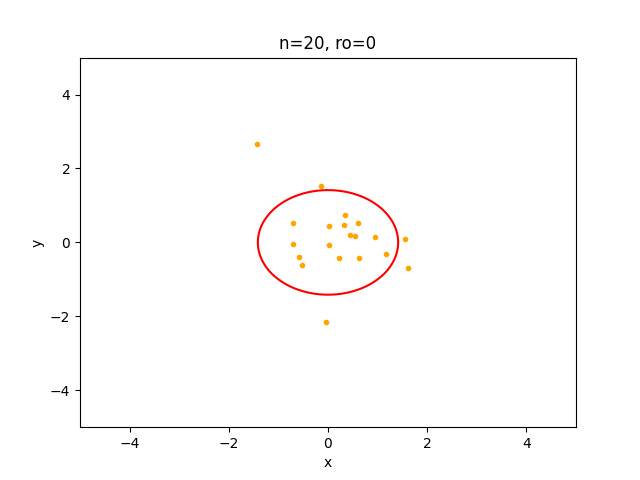
\includegraphics[scale=0.25]{n=20, ro=0}}
\caption{Эллипс рассеивания (\ref{eq:6}) и точки выборки нормального распределения (\ref{eq:2}) для $n = 20, \rho = 0$}
\end{figure}

\begin{figure}[h]
\center{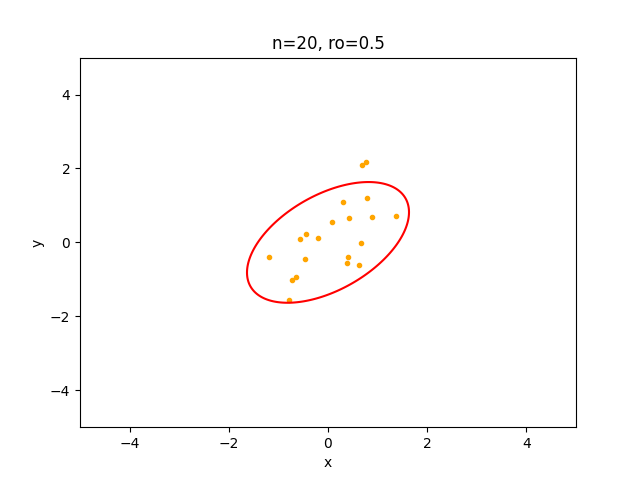
\includegraphics[scale=0.25]{n=20, ro=0.5}}
\caption{Эллипс рассеивания (\ref{eq:6}) и точки выборки нормального распределения (\ref{eq:2}) для $n = 20, \rho = 0.5$}
\end{figure}

\begin{figure}[h]
\center{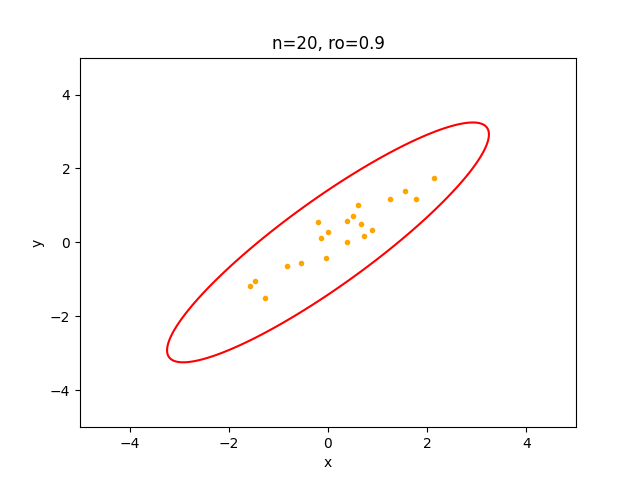
\includegraphics[scale=0.25]{n=20, ro=0.9}}
\caption{Эллипс рассеивания (\ref{eq:6}) и точки выборки нормального распределения (\ref{eq:2})  для $n = 20, \rho = 0.9$}
\end{figure}

\newpage
\begin{figure}[h]
\center{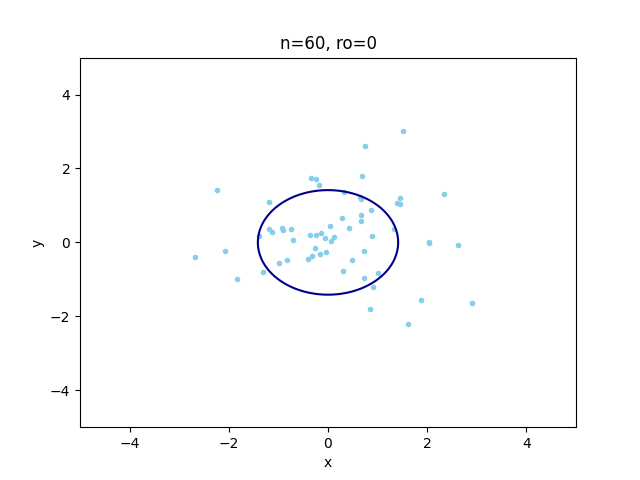
\includegraphics[scale=0.25]{n=60, ro=0}}
\caption{Эллипс рассеивания (\ref{eq:6}) и точки выборки нормального распределения (\ref{eq:2}) для $n = 60, \rho = 0$}
\end{figure}

\begin{figure}[h]
\center{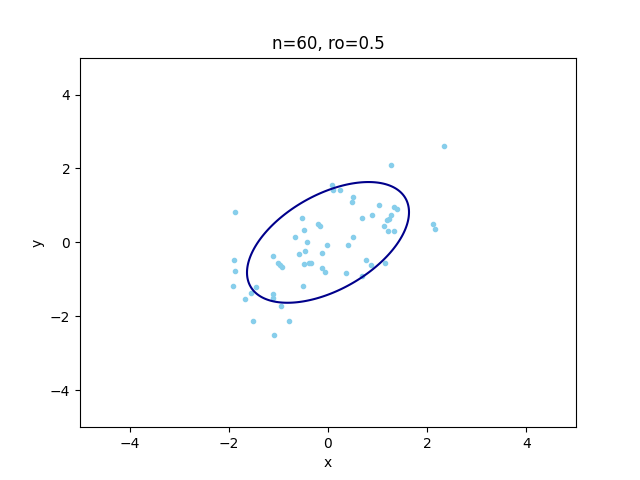
\includegraphics[scale=0.25]{n=60, ro=0.5}}
\caption{Эллипс рассеивания (\ref{eq:6}) и точки выборки нормального распределения (\ref{eq:2}) для $n = 60, \rho = 0.5$}
\end{figure}

\begin{figure}[h]
\center{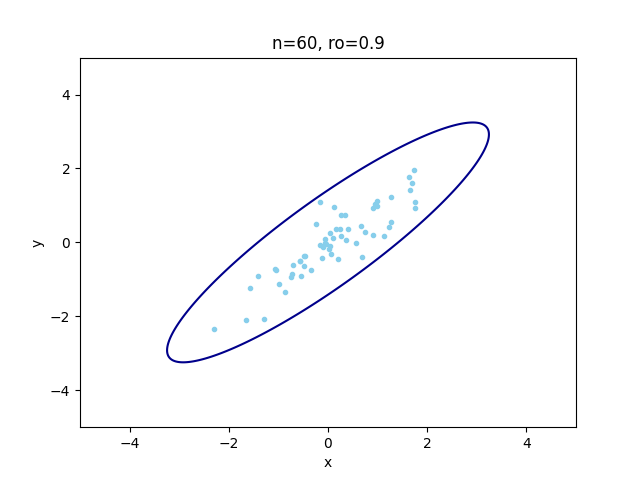
\includegraphics[scale=0.25]{n=60, ro=0.9}}
\caption{Эллипс рассеивания (\ref{eq:6}) и точки выборки нормального распределения (\ref{eq:2})  для $n = 60, \rho = 0.9$}
\end{figure}

\newpage
\begin{figure}[h]
\center{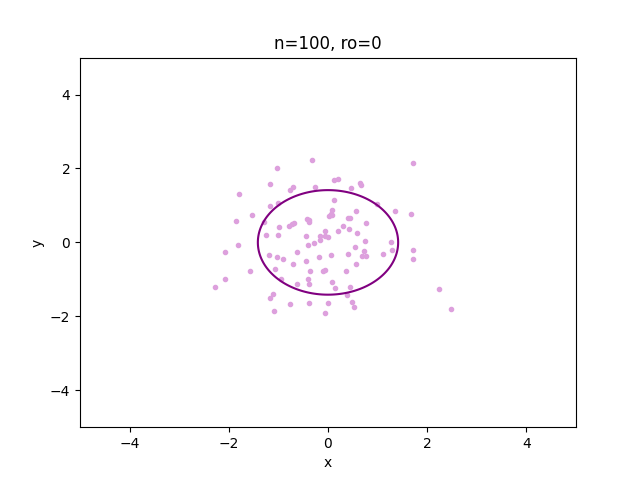
\includegraphics[scale=0.25]{n=100, ro=0}}
\caption{Эллипс рассеивания (\ref{eq:6}) и точки выборки нормального распределения (\ref{eq:2}) для $n = 100, \rho = 0$}
\end{figure}

\begin{figure}[h]
\center{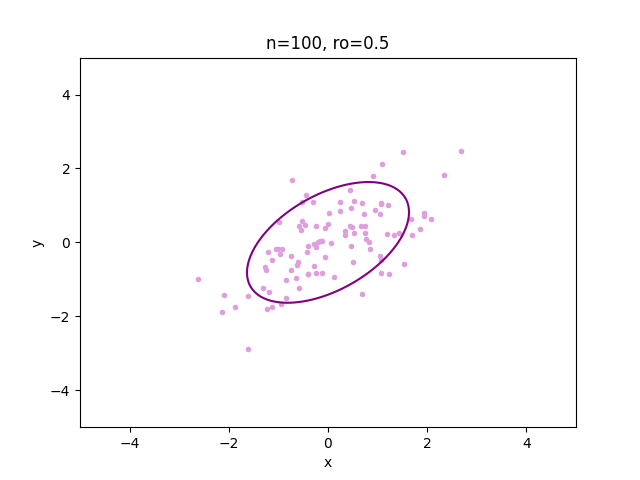
\includegraphics[scale=0.25]{n=100, ro=0.5}}
\caption{Эллипс рассеивания (\ref{eq:6}) и точки выборки нормального распределения (\ref{eq:2}) для $n = 100, \rho = 0.5$}
\end{figure}

\begin{figure}[h]
\center{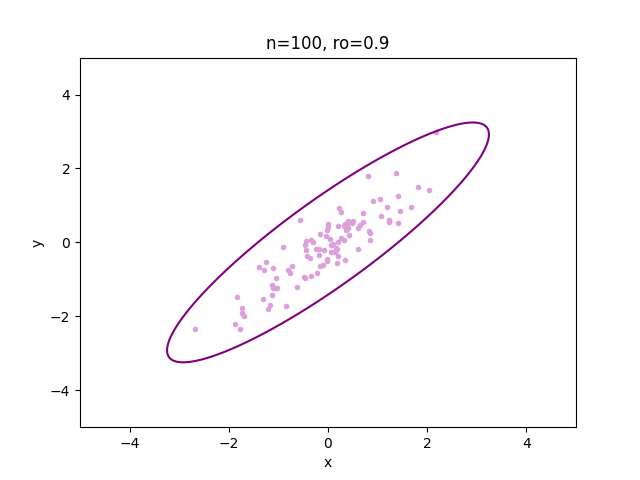
\includegraphics[scale=0.25]{n=100, ro=0.9}}
\caption{Эллипс рассеивания (\ref{eq:6}) и точки выборки нормального распределения (\ref{eq:2})  для $n = 100, \rho = 0.9$}
\end{figure}

\newpage
\section{Обсуждение}

\subsection{Выборочные коэффициенты корреляции}

Исходя из результатов пункта \ref{sec:1} для выборочных коэффициентов корреляции нормального распределения и из пункта \ref{sec:2} о смеси нормальных распределений можно сделать следующие выводы:

\begin{itemize}
	\item Для средних значений и средних значений квадрата характерно следующее неравенство: $r_Q < r_S < r$, исключением\footnote{Данное исключение наблюдается для нормального распределения} в некоторых случаях являются некоррелированные величины, т. е. с коэффициентом корреляции $\rho = 0$.
	\item Для дисперсиий же характерно соотношение $r_S < r_Q < r$, исключением также в некоторых случаях являются некоррелированные величины.
\end{itemize}

\subsection{Эллипс рассеивания}

Процент попавших элементов выборки в эллипс рассеивания (95\% - ная доверительная область) примерно равен его теоретическому значению (95\%)
\end{document}